%%
%% 2019 07 04 Ph. G. Freimann
%%

\section*{Einstiegsaufgabe}
\sectuntertitel{Der Anfang ist die Hälfte des Ganzen (Aristoteles)}
%%%%%%%%%%%%%%%%%%%%%%%%%%%%%%%%%%%%%%%%%%%%%%%%%%%%%%%%%%%%%%%%%%%%%%%%%%%%%%%%%
%%Lehrmittel:
%%\GESO{\cite{marthaler21alg} ab. S. 22}
%%\TALS{\cite{frommenwiler17alg} und \cite{frommenwiler18geom}}

\subsection*{Abholen des Bekannten und Geübten}

\TALS{\olatLinkPruefung{Einstiegstest}{https://olat.bbw.ch/auth/RepositoryEntry/572162090/CourseNode/106131924079692}}

\subsubsection*{Die Konservendose}
Stellen Sie sich vor, ein guter Freund von Ihnen stellt Konservendosen her.

Sie müssten für ihn eine optimale Dose in Form eines Kreiszylinders entwerfen, die möglichst wenig
Material benötigt.

\begin{center}
\raisebox{-1cm}{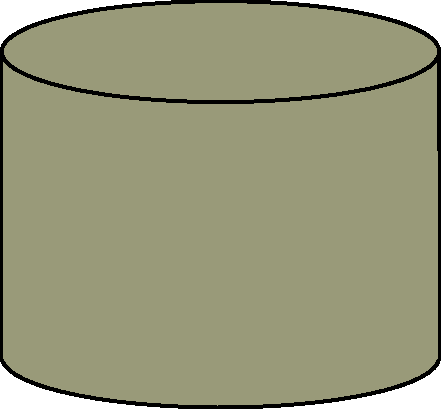
\includegraphics[width=5cm]{tals/010/img/Konservendose.pdf}}
\end{center}

Ihr Freund will exakt einen Liter
Zwiebelsuppe\footnote{S. \textit{Asterix} «Der Kupferkessel»} pro Dose abfüllen.

Wie hoch, wie breit (Radius/Durchmesser) muss die Dose nun sein,
damit \textbf{möglichst wenig Blech} verwendet wird? Was sind Ihre
Überlegungen dazu? Welche Formeln kennen Sie schon? Eine Näherung auf
5\% bis 10\% Genauigkeit sollte schon reichen; eine exakte Berechnung ist hier nicht gefordert.


\newpage
Platz für Ihre Überlegungen:
\TNTeop{
  Volumen = 1 Kubikdezimeter:

  $$r^2\pi \cdot{} h = 1 \text{ dm}^3$$

  $$\Longrightarrow h = \frac1{r^2\pi}$$

  Oberfläche:

  $$O = 2r\pi\cdot{}h + 2r^2\pi = 2r\pi\cdot{} \frac1{r^2\pi} +
  2r^2\pi = \frac2r + 2r^2\pi$$

  Minimieren = Ableitung = 0 setzen

  $$\frac{dO}{dr} = \frac{-2}{r^2} + 4r\pi \stackrel{!}{=} 0$$
  $$\Longrightarrow r^3 = \frac1{2\pi} \Longrightarrow
  r=\sqrt[3\,\,]{\frac1{2\pi}} \approx 0.541926 \Longrightarrow d=h\approx  1.08385 \text{ dm}$$

  Eine Näherung von 1.1 dm sollte hier aber bereits reichen: Eine
  Berechnung oder genauere Annäherung war nicht verlangt.
}

